\begin{appendices}
\clearpage
\pagenumbering{roman}	
\chapter{Periodensystem}
	
% http://commons.wikimedia.org/wiki/File:Periodic_table_simple_de_bw.svg
\begin{figure}\label{fig:persys}
	\centering
	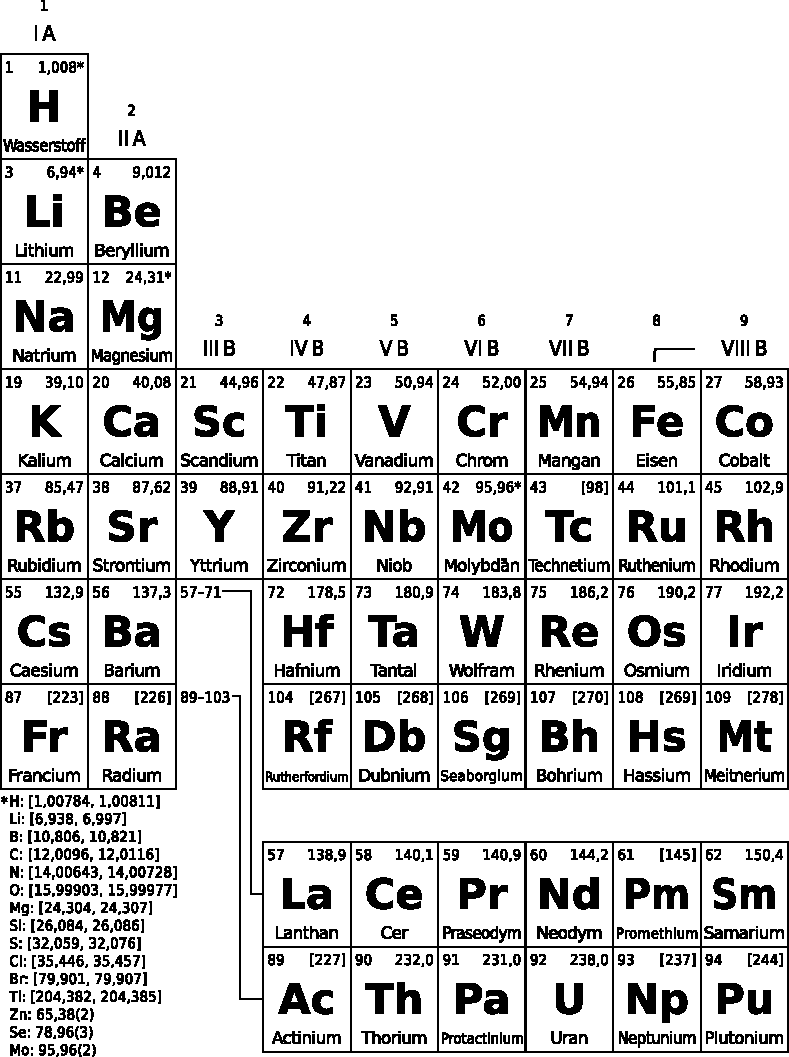
\includegraphics[width=\textwidth]{../fig/periodensystem_1.pdf}
\end{figure}	

\begin{figure}
	\centering
	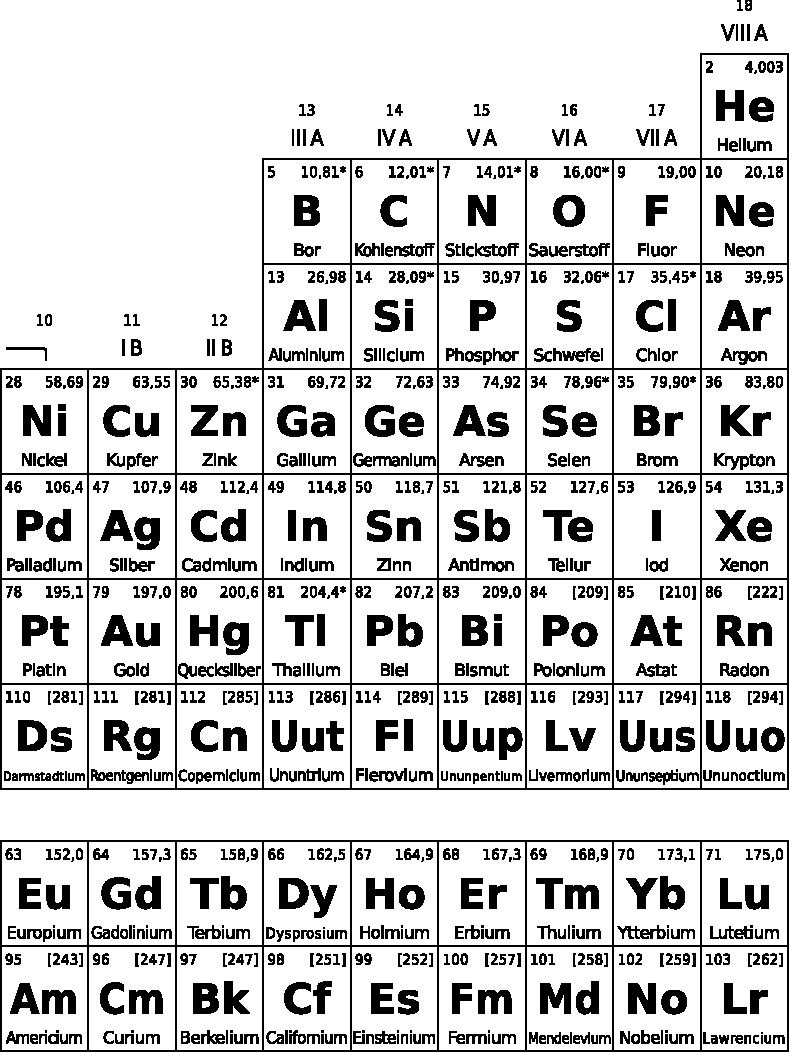
\includegraphics[width=\textwidth]{../fig/periodensystem_2.pdf}
\end{figure}

\chapter{Griechisches Alphabet}
\begin{table}[h!]
	\rowcolors{1}{lgray}{white}
	\begin{tabular}{c p{0.1\textwidth} p{0.3\textwidth} c p{0.1\textwidth} l}
		A & $\alpha$ & Alpha 			& N & $\nu$ & Ny \\
		B & $\beta$ & Beta 			& $\Xi$ & $\xi$ & Xi \\
		$\Gamma$ & $\gamma$ & Gamma 		& O & $o$ & Omikron \\
		$\Delta$ & $\delta$ & Delta 		& $\Pi$ & $\pi$ & Pi \\
		E & $\varepsilon$ ($\epsilon$) & Epsilon & P & $\rho$ ($\varrho$) & Rho \\
		Z & $\zeta$ & Zeta 			& $\Sigma$ & $\sigma$ ($\varsigma$) & Sigma \\
		H & $\eta$ & Eta 			& T & $\tau$ & Tau \\
		$\Theta$ & $\vartheta$ ($\theta$) & Theta & Y & $\upsilon$ & Ypsilon \\
		I & $\iota$ & Iota 			& $\Phi$ & $\varphi$ ($\phi$) & Phi \\
		K & $\kappa$ & Kappa 			& X & $\chi$ & Chi \\
		$\Lambda$ & $\lambda$ & Lambda 		& $\Psi$ & $\psi$ & Psi \\
		M & $\mu$ & My 				& $\Omega$ & $\omega$ & Omega \\
	\end{tabular}
\end{table}

\end{appendices}
